The authentication was also one of the interesting aspects for security, as it's a way to
prevent confidential data from being accessed without having the right credentials. But the 
prior used solution was having a permanent JWT token that is acquired during the login, meaning 
that once the that Token is generated it could be permanently used to access the data as it didn't
use any additional timing parameter to expire the token.

As for that, came the need to implement a ephemeral token, which is a token that gets expired after
a certain time, to access the data and opted to add a refreshing mechanism which was to make the
user experience better to avoid the need of having them reconnect within their sessions.

But not only that, we also opted to move from a Bearer token transportation of the token to a HTTP Only cookie,
which is a cookie that is only accessible through the HTTP protocol, not the Javascript and is proclaimed to
be the safest option to store the JWT. And then proceeded to embed the token within the cookie,
as so we can avoid the possiblity of exploitation through JS injections to acquire the token.

The authentication had a simple flow \ref{fig:token}, the user presented his credentials,
the server validated them, in case they were valid the server would generate a new access 
token, which was embedded in the header as a HTTP Only cookie then that would make 
all the request coming from the front end to the server to have the token in the header
with no need for the Javascript to do any handling for that last.

\begin{figure}[!htbp]
    \centering
    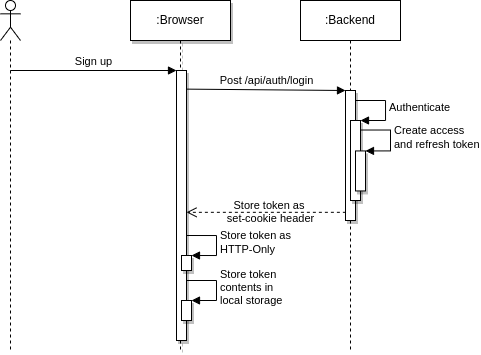
\includegraphics[width=0.75\textwidth]{images/JWTHttpOnly.png}
    \caption{\footnotesize{JWT HTTP Only Cookie}}
    \label{fig:token}
\end{figure}

The refresh token mechanism was to make the user experience better and also to increase
the security of the application, make the intercepted JWT tokens mostly come in useless
if they were caught late, as they would be expired.

So the flow \ref{fig:refresh} of that was to that during the login there was a generation
of access token and refresh token, the referesh token came in handy to create a new access
token once the old one has expired and the user was still active during that session, to
avoid forcing the user to re-login.

\begin{figure}[!htbp]
    \centering
    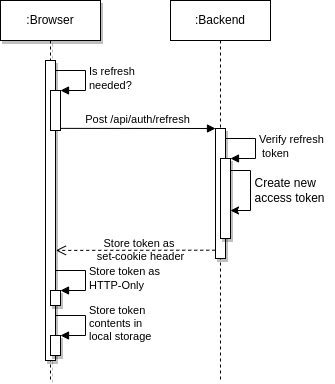
\includegraphics[width=0.42\textwidth]{images/refresh.png}
    \caption{\footnotesize{Refresh token}}
    \label{fig:refresh}
\end{figure}

\newpage
